\documentclass{sciposter}
\usepackage{lipsum}
\usepackage{epsfig}
\usepackage{amsmath}
\usepackage{amssymb}
\usepackage{multicol}
\usepackage{graphicx,url}
\usepackage{textpos}   
\usepackage[utf8]{inputenc}
\usepackage{xcolor}
\newtheorem{Def}{Definition}



\title{
\leavevmode{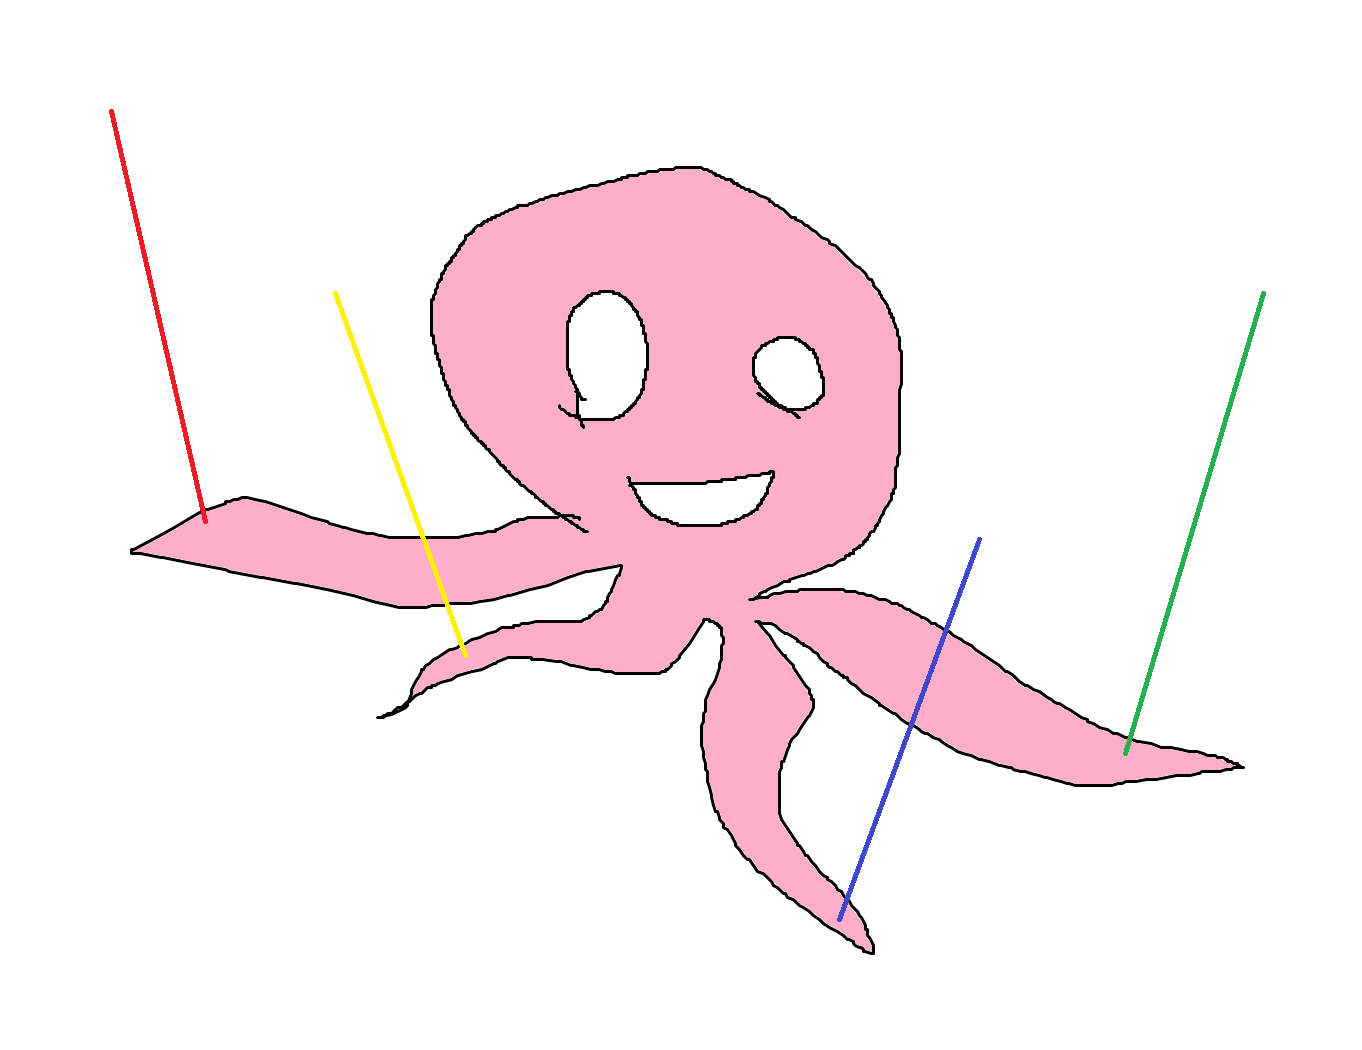
\includegraphics[width=0.5\textwidth]{Logos/gestikulaser.png}}\\
Gestikulaser}
%Título do projeto

\author{Christoph Behr, Cailing Fu, Nicole Grubert, Daniel Wolff}
%nome dos autores by the current \maketitle

%\renewcommand\printleftlogo
%  {\begin{center}
%     \resizebox{\textwidth}{!}%
%       {
\includegraphics{TOSLogo.png}
\includegraphics{COSIMALogo.png}}
%   \end{center}
%  }
  
%\rightlogo[2]{TOSLogo.png}
%\leftlogo[2]{COSIMALogo}

%Section title color:
\definecolor{SectionCol}{rgb}{0.0, 0.329411, 0.62353} % RWTH Blau
% Section block color:
\definecolor{BoxCol}{rgb}{0.949,0.949,0.949} % Grau

\begin{document}

% TOS Logo oben links
\begin{textblock*}{60px}(0cm,0cm)

\includegraphics[height=6cm,width=20cm]{Logos/TOS.png}
\end{textblock*}

% COSIMA18 Logo oben rechts
\begin{textblock*}{60px}(55cm,0mm)

\includegraphics[height=6cm,width=20cm]{Logos/Cosima18.png}
\end{textblock*}

\maketitle

%%% Begin of Multicols-Enviroment
\begin{multicols}{3}
\setlength{\parindent}{2em}

\section{Unsere Vision}
Was ist der Gestikulaser? 

\section{Die Beta-Version}
Foto von alter Photoplatte wo alles noch drauf geklebt ist etc.

%%% Introduction
\section{Photoplatte}
Beschreibung zur Photoplatte \\

% Einfügen eines Bildes
%\begin{figure}[h]
%\begin{center}
%
\includegraphics[width=10cm]{TOSLogo.png}
%\end{center}
%\end{figure}

\section{Oktokommander}
Hier kommt ein Text mit Bildern zum Oktokommander und wie dieser funktioniert.

\section{Detektormodul}
Hier werden die Detektormodule genau beschrieben.

\section{Ausblick}
Der Handschuh und das ganze modulare Zeug beschreiben.

\end{multicols}

\conference{\raisebox{0.5cm}[0cm]{
\includegraphics[height=3cm]{Logos/VDE.jpg} } \hfill
\raisebox{1.25cm}[0cm]{
\includegraphics[height=1.5cm]{Logos/Faulhaber.png}} \hfill
\raisebox{0cm}[0cm]{
\includegraphics[height=4cm]{Logos/micronit.jpg}} \hfill
\raisebox{0cm}[0cm]{
\includegraphics[height=4cm]{Logos/electronica.png}} \hfill 
\raisebox{0cm}[0cm]{
\includegraphics[height=4cm]{Logos/BMBF.jpg}}}

\end{document}